%!TEX root = ../NCVC.tex

\mysection{中級編}

\subsection{移動レイヤ}
 NCVCには,原点レイヤ・切削レイヤの他にあと3つのレイヤ情報を読み込む機能があります.
ここではそのうちの2つ,加工開始位置指示レイヤと強制移動指示レイヤを解説します.

\subsubsection{加工開始位置指示レイヤ}
 図\ref{fig:sample3.pdf} のような加工を考えます.
原点はワーク矩形左下で円を内側から螺旋状に切削したいのですが,これだけでは思ったようなGコードを生成できません.

 NCVCは次の切削データを検索するとき,現在位置に最も近い座標を検索します.
したがって,原点から一番近い座標である外側の座標からGコードの生成を始めます.

 これを回避するため,NCVCでは[加工開始位置指示レイヤ]を用意しています.
CADでの作図で原点・切削の両レイヤとは別のレイヤを用意し,円を1つ作図して下さい.
レイヤ名も設定です.作図方法は原点指示と同じ,円の中心が加工開始座標となります.

 NCVCでの設定は【\ref{sec:ReadCAD} CADデータの読み込み】と同じです.
[読み込みレイヤ2]のタブをクリックし,NCVCが読み込むレイヤ名を設定して下さい(図\ref{fig:ReadSetup3.png}).
[読み込みレイヤ2]の設定は必須ではありませんが,CAD側で意図的に作図しない限りNCVCは読み込みませんので,常にこの設定にしても問題ありません.
レイヤ名は,原点・切削の両レイヤと同様に任意です.CAD側の設定と合わせて下さい.
加工開始指示を指示したシミュレーション結果を図\ref{fig:sample3.png} に示します.

\begin{minipage}{0.5\textwidth}
\begin{figure}[H]
\centering
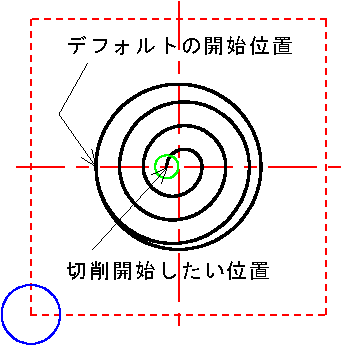
\includegraphics{No3/fig/move-crop.pdf}
\caption{サンプル図形}
\label{fig:sample3.pdf}
\end{figure}
\end{minipage}
\begin{minipage}{0.5\textwidth}
\begin{figure}[H]
\centering
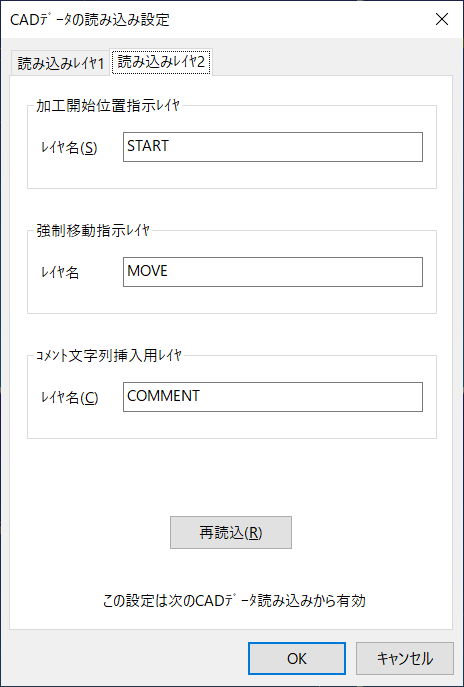
\includegraphics[scale=0.7]{No3/fig/ReadSetup3.png}
\caption{読み込みレイヤ設定}
\label{fig:ReadSetup3.png}
\end{figure}
\end{minipage}

\begin{figure}[H]
\centering
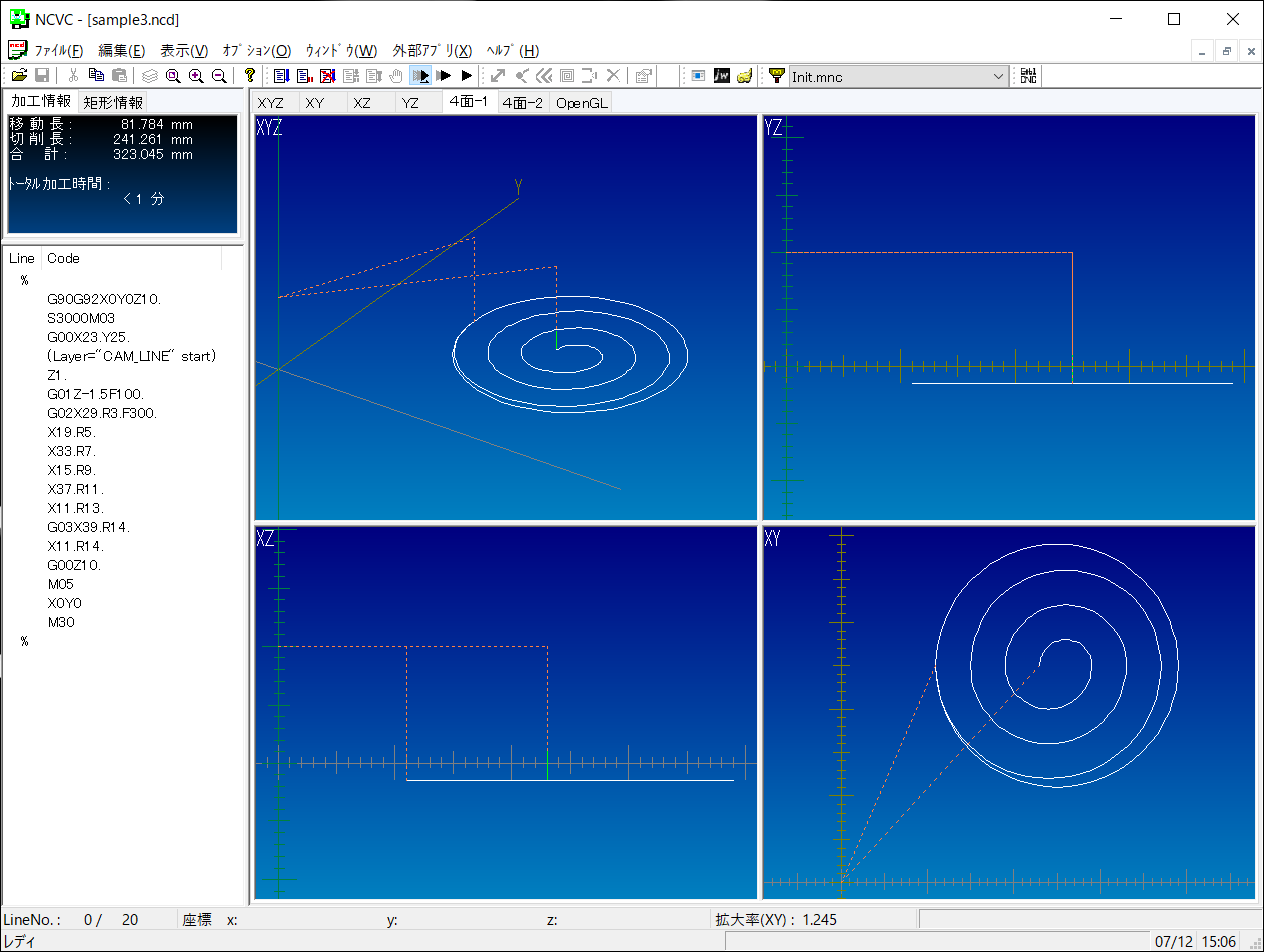
\includegraphics[scale=0.55]{No3/fig/sample3.png}
\caption{加工開始位置を追加したGコードシミュレーション画面}
\label{fig:sample3.png}
\end{figure}

 加工開始位置指示レイヤにはもう1つ機能があります.
例えば図\ref{fig:approach-img.png} のようなワーク形状の場合,原点からの最短移動ではワークに干渉してしまいます.
この場合,図\ref{fig:approach.pdf} のように干渉しないような移動軌跡を加工開始位置指示レイヤに作図することで,原点からの移動動作を制御することができます.
Z軸の初期座標を上げることで回避できる場合もあります.用途に応じてご使用下さい.

\begin{minipage}{0.5\textwidth}
\begin{figure}[H]
\centering
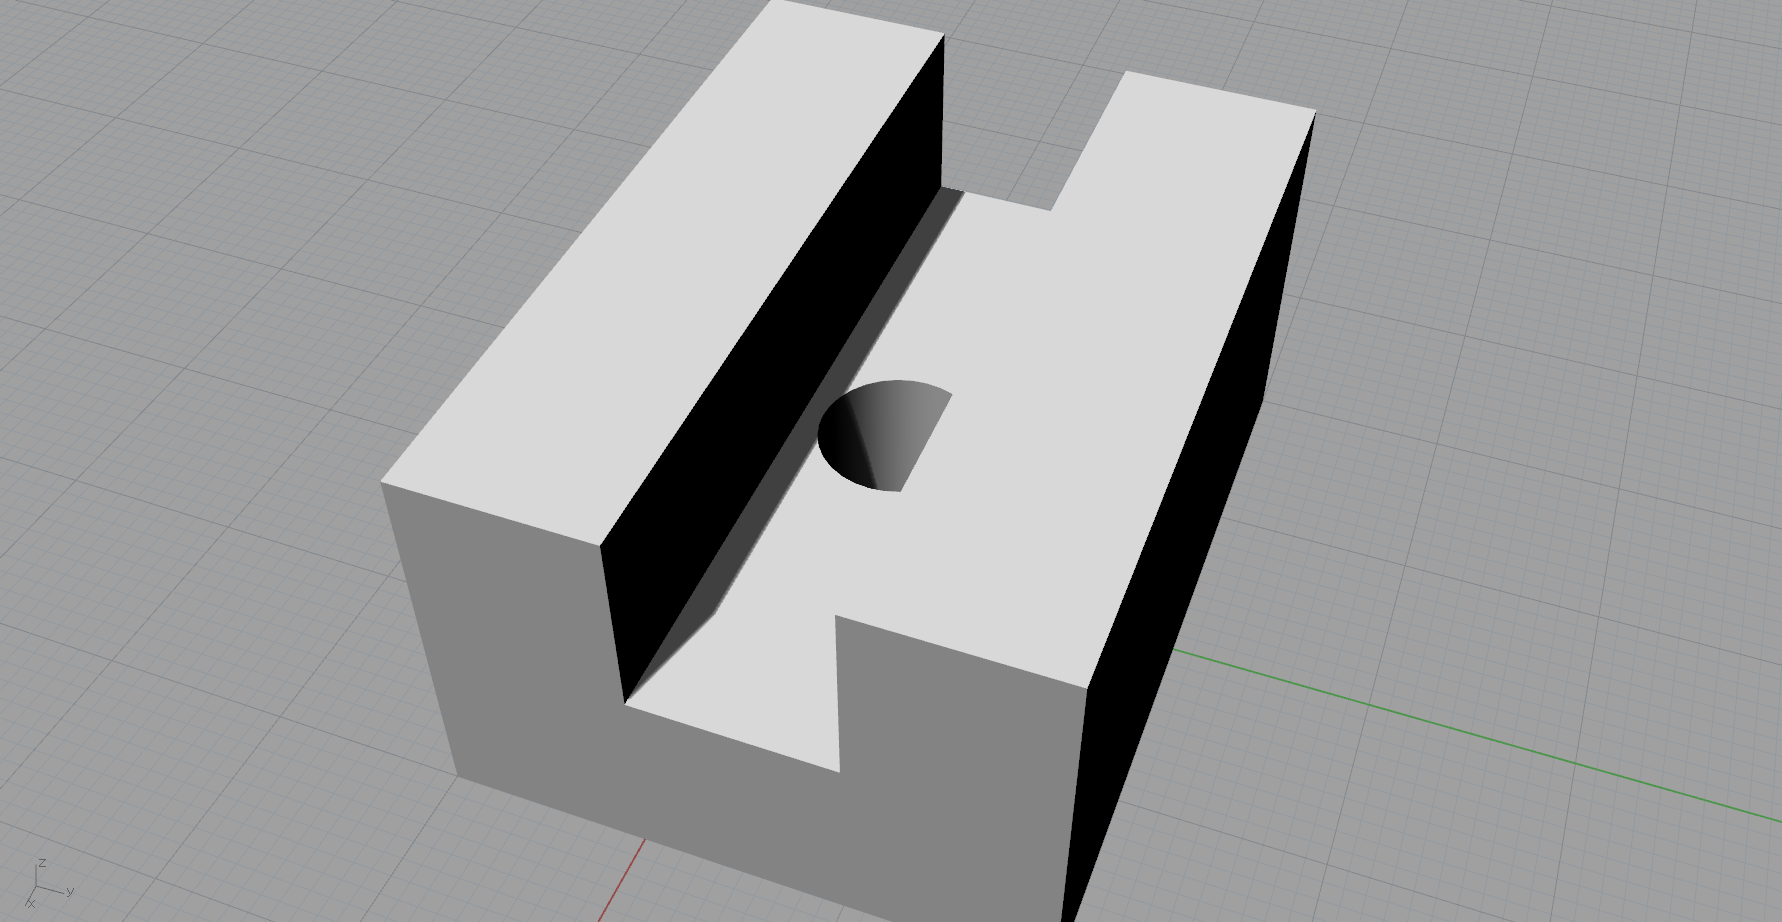
\includegraphics[width=\textwidth]{No3/fig/approach-img.png}
\caption{サンプルイメージ図}
\label{fig:approach-img.png}
\end{figure}
\end{minipage}
\begin{minipage}{0.5\textwidth}
\begin{figure}[H]
\centering
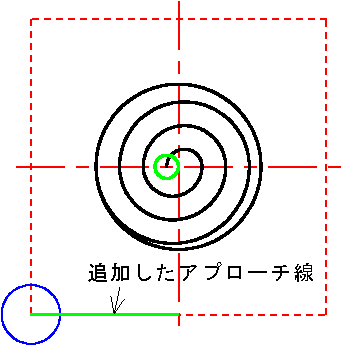
\includegraphics{No3/fig/approach-crop.pdf}
\caption{アプローチ線}
\label{fig:approach.pdf}
\end{figure}
\end{minipage}

\begin{figure}[H]
\centering
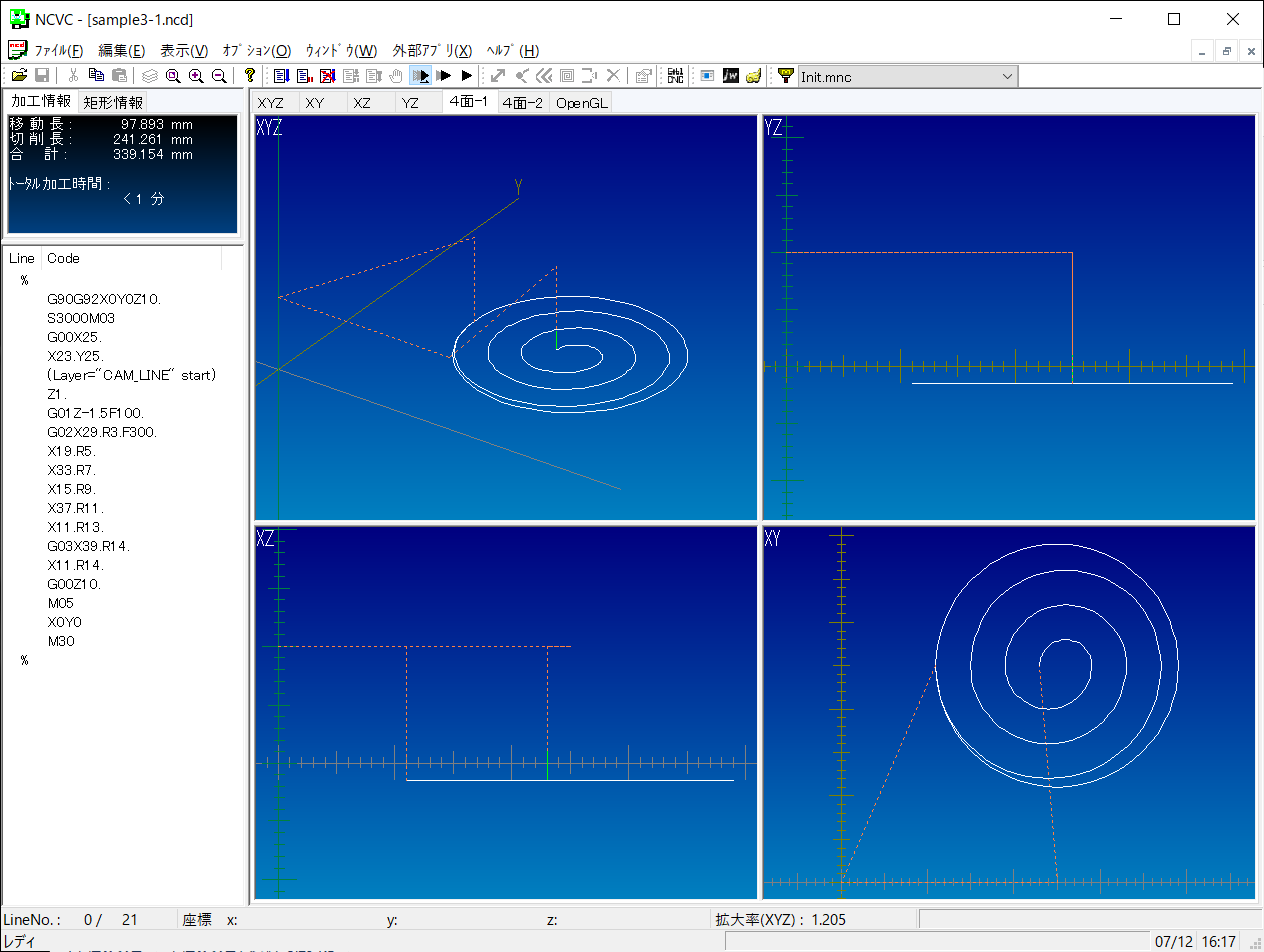
\includegraphics[scale=0.55]{No3/fig/sample3-1.png}
\caption{アプローチ線を追加したGコードシミュレーション画面}
\label{fig:sample3-1.png}
\end{figure}
